\section{Properties of Line Integrals}\label{sec:line_int_props}

We know from the previous section that for line integrals of real-valued functions (scalar fields), reversing the direction in which the integral is taken along a curve does not change the value of the line integral:
\[\int_C f(x,y)\,ds = \int_{-C} f(x,y)\,ds\]
For line integrals of vector fields, however, the value does change. To see this, let $\vecf(x,y) =P(x,y)\,\veci + Q(x,y)\,\vecj$ be a vector field, with $P$ and $Q$ continuously differentiable functions. Let $C$ be a smooth curve parametrized by $x=x(t)$, $y=y(t)$, $a \le t \le b$, with position vector $\vecr(t) = x(t)\,\veci + y(t)\,\vecj$ (we will usually abbreviate this by saying that $C: \vecr(t) = x(t)\,\veci + y(t)\,\vecj$ is a smooth curve). We know that the curve $-C$ traversed in the opposite direction is parametrized by $x=x(a+b-t)$, $y=y(a+b-t)$, $a \le t \le b$. Then
\begin{align*}
 \int_{-C} P(x,y)\,dx &= \int_a^b P(x(a+b-t),y(a+b-t))\,\frac{d}{dt}(x(a+b-t))\,dt\\
  &= \int_a^b P(x(a+b-t),y(a+b-t))\,(-x\,'(a+b-t))\,dt\text{ (by the Chain Rule)}\\
  &= \int_b^a P(x(u),y(u))\,(-x\,'(u))\,(-du)\text{ (by letting $u=a+b-t$)}\\
  &= \int_b^a P(x(u),y(u))\,x\,'(u)\,du\\
  &= -\int_a^b P(x(u),y(u))\,x\,'(u)\,du,\text{ since $\int_b^a = -\int_a^b$, so}\\
  \int_{-C} P(x,y)\,dx &= -\int_C P(x,y)\,dx
\end{align*}
since we are just using a different letter ($u$) for the line integral along $C$. A similar argument shows that
\[\int_{-C} Q(x,y)\,dy = -\int_C Q(x,y)\,dy ,\]
and hence
\begin{align*}
 \int_{-C} \vecf\cdot d\vecr
 &= \int_{-C} P(x,y)\,dx + \int_{-C} Q(x,y)\,dy\\
  &= -\int_C P(x,y)\,dx + -\int_C Q(x,y)\,dy\\
  &= -\left( \int_C P(x,y)\,dx + \int_C Q(x,y)\,dy \right)\\
  \int_{-C} \vecf\cdot d\vecr &= -\int_C \vecf\cdot d\vecr .
\end{align*}

The above formula can be interpreted in terms of the work done by a force $\vecf(x,y)$ (treated as a vector) moving an object along a curve $C$: the total work performed moving the object along $C$ from its initial point to its terminal point, and then back to the initial point moving backwards along the same path, is zero. This is because when force is considered as a vector, direction is accounted for.

The preceding discussion shows the importance of always taking the \emph{direction} of the curve into account when using line integrals of vector fields. For this reason, the curves in line integrals are sometimes referred to as \emph{directed curves} or \emph{oriented curves}.\index{directed curve}

Recall that our definition of a line integral required that we have \emph{a} parametrization $x=x(t)$, $y=y(t)$, $a \le t \le b$ for the curve $C$. But as we know, any curve has infinitely many parameterizations. So could we get a different value for a line integral using some other parametrization of $C$, say, $x=\tilde{x}(u)$, $y=\tilde{y}(u)$, $c \le u \le d$ ? If so, this would mean that our definition is not well-defined. Luckily, it turns out that the value of a line integral of a vector field is unchanged as long as the direction of the curve $C$ is preserved by whatever parametrization is chosen:

\theorem{thm:lineintreparam}{Line Integral is Independent of Parameterization}{Let $\vecf(x,y) = P(x,y)\,\veci + Q(x,y)\,\vecj$ be a vector field, and let $C$ be a smooth curve parametrized by $x=x(t)$, $y=y(t)$, $a \le t \le b$. Suppose that $t=\alpha(u)$ for $c \le u \le d$, such that $a=\alpha(c)$, $b=\alpha(d)$, and $\alpha\,'(u) > 0$ on the open interval $(c,d)$ (i.e., $\alpha(u)$ is strictly increasing on $[c,d]$). Then $\int_C \vecf\cdot d\vecr$ has the same value for the parameterizations $x=x(t)$, $y=y(t)$, $a \le t \le b$ and $x=\tilde{x}(u)=x(\alpha(u))$, $y=\tilde{y}(u)=y(\alpha(u))$, $c \le u \le d$.}

\begin{proof}
 Since $\alpha(u)$ is strictly increasing and maps $[c,d]$ onto $[a,b]$, then we know that $t=\alpha(u)$ has an inverse function $u=\alpha^{-1}(t)$ defined on $[a,b]$ such that $c=\alpha^{-1}(a)$, $d=\alpha^{-1}(b)$, and $\frac{du}{dt} = \frac{1}{\alpha\,'(u)}$. Also, $dt = \alpha\,'(u)\,du$, and by the Chain Rule
 \[
  \tilde{x}\,'(u) = \frac{d\tilde{x}}{du} = \frac{d}{du}(x(\alpha(u))) = \frac{dx}{dt}\,\frac{dt}{du} =
  x\,'(t)\,\alpha\,'(u) \quad\Rightarrow\quad x\,'(t) = \frac{\tilde{x}\,'(u)}{\alpha\,'(u)}
 \]
 so making the substitution $t=\alpha(u)$ gives
 \begin{align*}
  \int_a^b P(x(t),y(t))\,x\,'(t)\,dt &=
   \int_{\alpha^{-1}(a)}^{\alpha^{-1}(b)} P(x(\alpha(u)),y(\alpha(u)))\,\frac{\tilde{x}\,'(u)}{\alpha\,'(u)}
   \,(\alpha\,'(u)\,du)\\
   &= \int_c^d P(\tilde{x}(u),\tilde{y}(u))\,\tilde{x}\,'(u)\,du ,
 \end{align*}
 which shows that $\int_C P(x,y)\,dx$ has the same value for both parameterizations. A similar argument shows that $\int_C Q(x,y)\,dy$ has the same value for both parameterizations, and hence $\int_C \vecf\cdot d\vecr$
 has the same value.
\end{proof}

Notice that the condition $\alpha\,'(u) > 0$ in \autoref{thm:lineintreparam} means that the two parameterizations move along $C$ in the same direction. That was \emph{not} the case with the ``reverse'' parametrization for $-C$: for $u=a+b-t$ we have $t=\alpha(u)=a+b-u \Rightarrow \alpha\,'(u) = -1 <0$.

\example{ex_line_int_again}{Re-evaluating a Line Integral}{Evaluate the line integral $\int_C (x^2 + y^2 )\,dx + 2xy\,dy$ from \autoref{exmp_lineintexmp} in \autoref{sec:line_int}, along the curve $C: x=t$, $y=2t^2$, $0 \le t \le 1$, where $t=\sin u$ for $0 \le u \le \pi/2$.}{First, we notice that $0=\sin 0$, $1=\sin (\pi/2)$, and $\frac{dt}{du} = \cos u > 0$ on $(0,\pi/2)$. So by \autoref{thm:lineintreparam} we know that if $C$ is parametrized by
 \[x=\sin u ,\quad y = 2\sin^2 u ,\quad 0 \le u \le \pi/2\]
 then $\int_C (x^2 + y^2 )\,dx + 2xy\,dy$ should have the same value as we found in \autoref{exmp_lineintexmp}, namely $\frac{13}{3}$. And we can indeed verify this:
 \begin{align*}
  \int_C (x^2 + y^2 )&\,dx + 2xy\,dy\\
   &= \int_0^{\pi/2} \left( (\sin^2 u + (2\sin^2 u)^2) \cos u +
   2(\sin u)(2\sin^2 u) 4\sin u \, \cos u \right)\,du\\
   &= \int_0^{\pi/2} \left( \sin^2 u + 20\sin^4 u \right) \cos u\,du\\
   &= \left.\frac{\sin^3 u}{3} + 4\sin^5 u \,\right|_0^{\pi/2}\\
   &= \frac{1}{3} + 4 = \frac{13}{3}
 \end{align*}
 In other words, the line integral is unchanged whether $t$ or $u$ is the parameter for $C$.}

By a \textbf{closed curve}, we mean a curve $C$ whose initial point and terminal point are the same, i.e. for $C$: $x=x(t)$, $y=y(t)$, $a \le t \le b$, we have $(x(a),y(a)) = (x(b),y(b))$.\index{closed curve}

\noindent\begin{minipage}[t]{\linewidth}\noindent%
\captionsetup{type=figure}%
 \centering
 \begin{tabular}{cc}
 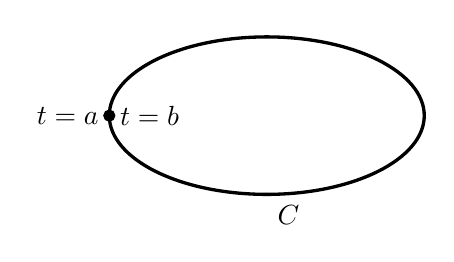
\begin{tikzpicture}
  \usetikzlibrary{arrows}
  \fill[draw={\colorone},fill={\colorone}] (-2,0) circle (2pt);
  \draw [draw={\colorone},very thick] (-2,0)
   node[left]{$t=a$}node[right]{$t=b$}
   arc (180:90:2 and 1) node {\large $\blacktriangleright$};
  \draw [draw={\colorone},very thick] (0,1) arc (90:-90:2 and 1)
   node {\large $\blacktriangleleft$}node[below right]{$C$};
  \draw [draw={\colorone},very thick] (0,-1) arc (-90:-180:2 and 1);
 \end{tikzpicture}
  &
 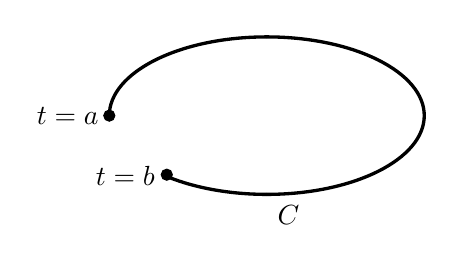
\begin{tikzpicture}
  \usetikzlibrary{arrows}
  \fill[draw={\colorone},fill={\colorone}] (-2,0) circle (2pt);
  \fill[draw={\colorone},fill={\colorone}] (-1.27,-0.75) circle (2pt);
  \draw [draw={\colorone},very thick] (-2,0)
   node[left]{$t=a$} arc (180:90:2 and 1) node {\large $\blacktriangleright$};
  \draw [draw={\colorone},very thick] (0,1) arc (90:-90:2 and 1)
   node {\large $\blacktriangleleft$}node[below right]{$C$};
  \draw [draw={\colorone},very thick] (0,-1) arc (-90:-130:2 and 1)
   node[left]{$t=b$};
 \end{tikzpicture} \\
 (a) Closed & (b) Not Closed
 \end{tabular}
 \caption{Closed vs nonclosed curves}
 \label{fig:closedcurve}
\end{minipage}

A \textbf{simple closed curve} is a closed curve which does not intersect itself. Note that any closed curve can be regarded as a union of simple closed curves (think of the loops in a figure eight). We use the special notation
\[\oint_C f(x,y)\,ds \quad\text{and}\quad \oint_C \vecf\cdot d\vecr\]
to denote line integrals of scalar and vector fields, respectively, along closed curves.\index{simple closed curve}\index{$\oint_C$} In some older texts you may see the notation $\;\ds\ointctrclockwise\;$ or $\;\ds\ointclockwise\;$ to indicate a line integral traversing a closed curve in a counterclockwise or clockwise direction, respectively.

So far, the examples we have seen of line integrals (e.g., \autoref{exmp_lineintexmp}) have had the same value for different curves joining the initial point to the terminal point. That is, the line integral has been independent of the path joining the two points. As we mentioned before, this is not always the case. The following theorem gives a necessary and sufficient condition for this \emph{path independence}:\index{path independence}

\theorem{thm:lineintpathindep}{Path Independence of Line Integrals}{In a region $R$, the line integral $\int_{C}\vecf\cdot d\vecr$ is independent of the path between any two points in $R$ if and only if $\oint_{C}\vecf\cdot d\vecr = 0$ for every closed curve $C$ which is contained in $R$.}

\begin{proof}
Suppose that
\mtable{The idea of proving \autoref{thm:lineintpathindep}.}{fig_path_indep}{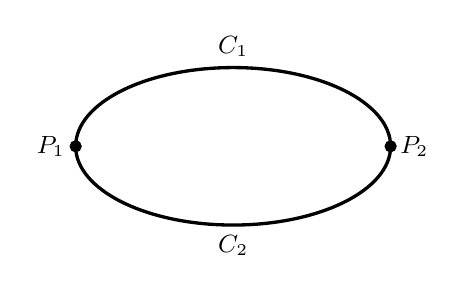
\begin{tikzpicture}
  \usetikzlibrary{arrows}
  \fill[draw={\colorone},fill={\colorone}] (-2,0) circle (2pt);
  \fill[draw={\colorone},fill={\colorone}] (2,0) circle (2pt);
  \draw [draw={\colorone},very thick] (-2,0)node[left]{\small$P_1$}
   arc (180:90:2 and 1) node {\large $\blacktriangleright$}node[above]{\small$C_1$};
  \draw [draw={\colorone},very thick] (0,1) arc (90:-90:2 and 1)
   node {\large $\blacktriangleright$}node[below]{\small$C_2$};
  \draw [draw={\colorone},very thick] (0,-1) arc (-90:-180:2 and 1);
  \node [right] at (2,0) {\small $P_2$};
 \end{tikzpicture}}
$\oint_{C}\vecf\cdot d\vecr = 0$ for every closed curve $C$  which is contained in $R$. Let $P_1$ and $P_2$ be two distinct points in $R$. Let $C_1$ be a curve in $R$ going from $P_1$ to $P_2$, and let $C_2$ be another curve in $R$ going from $P_1$ to $P_2$, as in \autoref{fig_path_indep}.

 
Then $C = C_1\cup -C_2$ is a closed curve in $R$ (from $P_1$ to $P_1$), and so $\oint_{C}\vecf\cdot d\vecr = 0$. Thus,
\begin{align*}
  0 &= \oint_{C}\vecf\cdot d\vecr\\[6pt]
  &= \int_{C_1}\vecf\cdot d\vecr + \int_{-C_2}\vecf\cdot d\vecr\\[6pt]
  &= \int_{C_1}\vecf\cdot d\vecr - \int_{C_2}\vecf\cdot d\vecr,\text{ and so}
\end{align*}
$\int_{C_1}\vecf\cdot d\vecr = \int_{C_2}\vecf\cdot d\vecr$. This proves path independence.

Conversely, suppose that the line integral $\int_{C}\vecf\cdot d\vecr$ is independent of the path between any two points in $R$. Let $C$ be a closed curve contained in $R$. Let $P_1$ and $P_2$ be two distinct points on $C$. Let $C_1$ be a part of the curve $C$ that goes from $P_1$ to $P_2$, and let $C_2$ be the remaining part of $C$ that goes from $P_1$ to $P_2$, again as in \autoref{fig_path_indep}. Then by path independence we have
 \begin{align*}
  \int_{C_1}\vecf\cdot d\vecr &= \int_{C_2}\vecf\cdot d\vecr\\[6pt]
  \int_{C_1}\vecf\cdot d\vecr - \int_{C_2}\vecf\cdot d\vecr &= 0\\[6pt]
  \int_{C_1}\vecf\cdot d\vecr + \int_{-C_2}\vecf\cdot d\vecr &= 0 ,\text{ so}\\[6pt]
  \oint_{C}\vecf\cdot d\vecr &= 0
 \end{align*}
 since $C = C_1\cup -C_2$ .
\end{proof}

Clearly, the above theorem does not give a practical way to determine path independence, since it is impossible to check the line integrals around all possible closed curves in a region. What it mostly does is give an idea of the way in which line integrals behave, and how seemingly unrelated line integrals can be related (in this case, a specific line integral between two points and \emph{all} line integrals around closed curves).
%
%For a more practical method for determining path independence, we first need a version of the Chain Rule for multivariable functions:\index{Chain Rule}
%
%\theorem{thm:chainrule2}{Chain Rule}{If $z=f(x,y)$ is a continuously differentiable function of $x$ and $y$, and both $x=x(t)$ and $y=y(t)$ are differentiable functions of $t$, then $z$ is a differentiable function of $t$, and
% \begin{equation}\label{eqn:chainrule2}
%  \frac{dz}{dt} = \frac{\partial z}{\partial x}\,\frac{dx}{dt} + \frac{\partial z}{\partial y}\,\frac{dy}{dt}
% \end{equation}
% at all points where the derivatives on the right are defined.}
%
%The proof is virtually identical to the proof of \autoref{thm:dirderiv} from Section 2.4 (which uses the Mean Value Theorem), so we omit it. (See \cite[\S\,6.5]{tm}.)
%We will now use this Chain Rule to
We will now prove the following \emph{sufficient} condition for path independence of line integrals:
% should we introduce ``simply connected''?

% todo Where does Theorem 135 require simply connected?
\theorem{thm:lineintsuffpath}{Fundamental Theorem of Line Integrals}{Let $\vecf(x,y) = P(x,y)\,\veci + Q(x,y)\,\vecj$ be a vector field in some region $R$ without holes, with $P$ and $Q$ continuously differentiable functions on $R$. Let $C$ be a smooth curve in $R$ parametrized by $x=x(t)$, $y=y(t)$, $a \le t \le b$. Suppose that there is a real-valued function $F(x,y)$ such that $\nabla F = \vecf$ on $R$. Then
\[\int_{C}\vecf\cdot d\vecr = F(B) - F(A) ,\]
where $A=(x(a),y(a))$ and $B=(x(b),y(b))$ are the endpoints of $C$. Thus, the line integral is independent of the path between its endpoints, since it depends only on the values of $F$ at those endpoints.}

\begin{proof}
 By definition of $\int_{C}\vecf\cdot d\vecr$, we have
 \begin{align*}
  \int_{C}\vecf\cdot d\vecr
  &= \int_a^b \Bigl( P(x(t),y(t))\,x\,'(t) + Q(x(t),y(t))\,y\,'(t) \Bigr)\,dt\\
  &= \int_a^b \left( \frac{\partial F}{\partial x}\,\frac{dx}{dt} + \frac{\partial F}{\partial y}\,\frac{dy}{dt}
   \right)\,dt \text{ (since $\nabla F = \vecf \Rightarrow \frac{\partial F}{\partial x} = P$ and
  $\frac{\partial F}{\partial y} = Q$)}\\
  &= \int_a^b F\,'(x(t),y(t))\,dt \text{ (by \autoref{thm:multi_chain})}\\
  &= \left.F(x(t),y(t)) \,\right|_a^b = F(B) - F(A)
 \end{align*}
 by the Fundamental Theorem of Calculus.
\end{proof}

\autoref{thm:lineintsuffpath} can be thought of as the line integral version of the Fundamental Theorem of Calculus. A real-valued function $F(x,y)$ such that $\nabla F(x,y) = \vecf(x,y)$ is called a \textbf{potential} for \vecf. A \textbf{conservative} vector field is one which has a potential.\index{potential}

\youtubeVideo{62oBGKSjYiY}{Ex 1: Fundamental Theorem of Line Integrals --- Given Vector Field in a Plane}

\example{exmp_lineintexmpclosed}{Using the Fundamental Theorem of Line Integrals}{Recall from Examples \ref{exmp_lineintexmp}  and \ref{exmp_lineintexmppoly} in \autoref{sec:line_int} that the line integral $\int_C (x^2 + y^2 )\,dx + 2xy\,dy$ was found to have the value $\frac{13}{3}$ for three different curves $C$ going from the point $(0,0)$ to the point $(1,2)$. Use \autoref{thm:lineintsuffpath} to show that this line integral is indeed path independent.}{We need to find a real-valued function $F(x,y)$ such that
 \[
  \frac{\partial F}{\partial x}
  = x^2 + y^2 \quad\text{and}\quad \frac{\partial F}{\partial y} =  2xy .
 \]
 Suppose that $\frac{\partial F}{\partial x} = x^2 + y^2$, Then we must have $F(x,y) = \frac{1}{3}x^3 + xy^2 + g(y)$ for some function $g(y)$. So $\frac{\partial F}{\partial y} = 2xy + g\,'(y)$ satisfies the condition $\frac{\partial F}{\partial y} = 2xy$ if $g\,'(y)=0$, i.e., $g(y)=K$, where $K$ is a constant. Since any choice for $K$ will do (why?), we pick $K=0$. Thus, a potential $F(x,y)$ for  $\vecf(x,y) = ( x^2 + y^2 )\,\veci + 2xy\,\vecj$ exists, namely
 \[F(x,y) = \frac{1}{3}x^3 + xy^2 .\]
 Hence the line integral $\int_C (x^2 + y^2 )\,dx + 2xy\,dy$ is path independent.\index{conservative field}
 
Note that we can also verify that the value of the line integral of \vecf\ along any curve $C$ going from $(0,0)$ to $(1,2)$ will always be $\frac{13}{3}$, since by \autoref{thm:lineintsuffpath}
 \[
  \int_{C}\vecf\cdot d\vecr = F(1,2) - F(0,0) = \frac{1}{3}(1)^3 + (1)(2)^2 - (0+0) = \frac{1}{3} + 4 = \frac{13}{3} .
 \]}

A consequence of \autoref{thm:lineintsuffpath} in the special case where $C$ is a closed curve, so that the endpoints $A$ and $B$ are the same point, is the following:

\theorem{cor:lineintsuffpath}{Closed Line Integrals of Conservative Fields}{If a vector field $\vecf$ has a potential in a region $R$ without holes, then $\ds\oint_{C}\vecf\cdot d\vecr = 0$ for any closed curve $C$ in $R$ (i.e., $\ds\oint_{C}\nabla F\cdot d\vecr = 0$ for any real-valued function $F(x,y)$).}

\example{ex_use_cor}{Calculating a Closed Line Integral of a Conservative Field}{Evaluate $\ds\oint_C x\,dx + y\,dy$ for $C:$ $x=2\cos t$, $y=3\sin t$, $0\le t\le 2\pi$.}{The vector field $\vecf(x,y) = x\,\veci + y\,\vecj$ has a potential $F(x,y)$:
 \begin{align*}
  \frac{\partial F}{\partial x} = x &\Rightarrow F(x,y) = \frac{1}{2}x^2 + g(y) ,\text{so}\\
  \frac{\partial F}{\partial y} = y &\Rightarrow g\,'(y) = y \Rightarrow g(y) = \frac{1}{2}y^2 + K
 \end{align*}
 for any constant $K$, so $F(x,y) = \dfrac{1}{2}x^2 + \dfrac{1}{2}y^2$ is a potential for $\vecf(x,y)$. Thus,
 \[\oint_C x\,dx + y\,dy = \oint_{C}\vecf\cdot d\vecr = 0\]
 by \autoref{cor:lineintsuffpath}, since the curve $C$ is closed (it is the ellipse
 $\frac{x^2}{4}+\frac{y^2}{9}=1$).}

\printexercises{exercises/14_Line_Int_Props_exercises}
